La estructura organizacional del área de mantenimiento de SKYFILMS se ha diseñado para asegurar un flujo jerárquico claro cumplimiento de los requisitos establecidos por la Unidad Administrativa Especial de Aeronáutica Civil (Aerocivil) para explotadores de Sistemas de Aeronaves No Tripuladas (UAS), conforme al RAC 100.\\

El objetivo de esta estructura es garantizar que las decisiones técnicas relacionadas con el mantenimiento y la aeronavegabilidad continuada sean adoptadas por personal competente y autorizado, evitando conflictos de interés entre las áreas operativas y de control técnico.
La estructura organizacional también define con precisión las funciones, responsabilidades y autoridad de cada cargo vinculado al proceso de mantenimiento.

\section{Estructura Organizacional}
El área técnica de SKYFILMS está compuesta por los siguientes niveles jerárquicos:

\subsection{Descripción general de la estructura}
El área de mantenimiento de SKYFILMS está compuesta por los siguientes niveles jerárquicos y de responsabilidad:

\begin{itemize}

    \item \textbf{Gerente General}
    \item \textbf{Técnico UAS} (corresponde al Responsable de Mantenimiento del Manual de Operaciones)

\end{itemize}

Estos cargos conforman la estructura técnica mínima requerida para garantizar la operación segura y la gestión efectiva del mantenimiento. El Jefe de Pilotos UAS y el Gerente SMS (SMS) (en adelante, Gerente SMS) apoyan el proceso desde sus propias funciones, como se describe a continuación, y no forman parte de la cadena de liberación de aeronaves.

\subsection{Perfil y competencias del Técnico UAS}
\begin{itemize}
    \item Formación técnica o experiencia demostrable en aeronaves no tripuladas, electrónica o mecánica, verificada por el Gerente General antes de su designación. Su autorización inicial y sus límites están en el capítulo de capacidad técnica del personal.
    \item Entrenamiento inicial y recurrente según el capítulo de capacidad técnica del personal, y entrenamiento específico en el Mavic 4 Pro y en el Pavo20 Pro II.
    \item Conocimiento del RAC 100, del Manual de Operaciones, del SMS y de este Manual.
    \item Es la única persona autorizada para liberar una aeronave al servicio. Si no está disponible, no se libera ninguna aeronave y el mantenimiento se realiza con un proveedor aceptado (capítulo de proveedores). El Gerente General puede designar por escrito un reemplazo temporal que cumpla este perfil.
\end{itemize}

\subsection{Representación gráfica}
La estructura jerárquica y funcional se representa de la siguiente manera:

\begin{figure}[H]
\centering
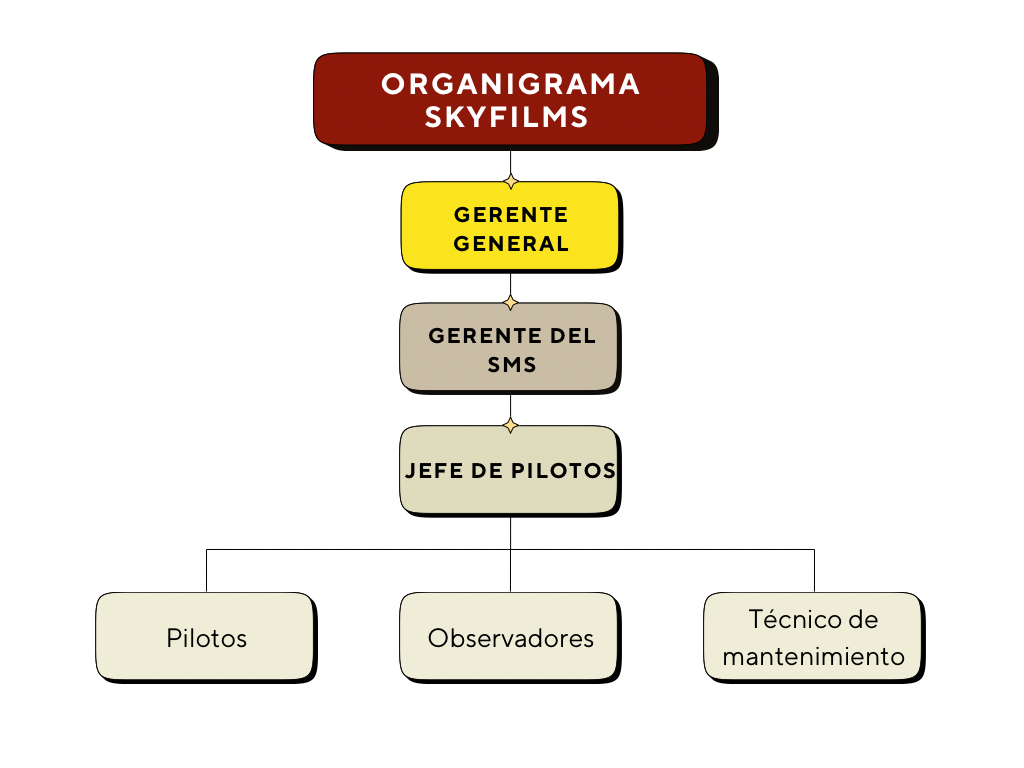
\includegraphics[width=.85\textwidth]{Imagenes/organigrama_skyfilm.PNG}
\caption{Estructura MCM Skyfilms}
\end{figure}


Esta representación refleja las líneas de autoridad, coordinación e intercambio de información entre las áreas de mantenimiento, seguridad operacional y operaciones de vuelo.

\section{Funciones y Responsabilidades del Personal}

\begin{enumerate}
    \item \textbf{Gerente General}
        \begin{itemize}
            \item Garantizar que la organización cumpla con las disposiciones del RAC 100 y con las políticas definidas por la Aerocivil.
            \item Aprobar el Manual de Control de Mantenimiento y sus revisiones.
            \item Asignar los recursos humanos, financieros y técnicos necesarios para el cumplimiento del Programa de Mantenimiento.
            \item Asegurar la coordinación efectiva entre las áreas de Mantenimiento, Operaciones y Seguridad Operacional.
            \item Mantener comunicación directa con la Aerocivil respecto a los temas de mantenimiento, enmiendas al MCM y cumplimiento regulatorio.
            \item Actuar como directivo responsable: responde ante la Aerocivil por que Skyfilms cumpla lo que dice este Manual y por que existan los recursos para ejecutarlo.
        \end{itemize}
    \item \textbf{Tecnico UAS}
        \begin{itemize}
            \item \textbf{Ejecución técnica:} Realizar inspecciones, mantenimientos, pruebas funcionales y calibraciones según los programas aprobados, asegurando la aeronavegabilidad de los UAS.

            \item \textbf{Registro y trazabilidad:} Diligenciar correctamente los formatos de mantenimiento, libros técnicos y reportes de servicio, garantizando la veracidad y oportunidad de la información registrada.

            \item \textbf{Uso adecuado de herramientas:} Emplear únicamente equipos, instrumentos y materiales certificados y en condiciones óptimas.

            \item \textbf{Cumplimiento normativo:} Aplicar los procedimientos, políticas de seguridad operacional y estándares técnicos establecidos por SKYFILMS y la Aerocivil.

            \item \textbf{Gestión de seguridad:} Reportar de manera inmediata cualquier hallazgo, daño o condición insegura que afecte la operación o el mantenimiento.

            \item \textbf{Apoyo en la gestión técnica:} Colaborar en la actualización del inventario de herramientas, componentes y registros técnicos bajo supervisión del Jefe de Pilotos y del Gerente General.

            \item \textbf{Control documental:} Asegurar que todos los documentos utilizados correspondan a versiones vigentes y que los registros se archiven conforme al sistema de gestión documental del MCM.

            \item \textbf{Factores humanos:} Mantener condiciones físicas y mentales adecuadas para el desempeño de sus labores, evitando trabajar bajo fatiga, estrés o presión excesiva.
        \end{itemize}
    \item \textbf{Gerente SMS}
        \begin{itemize}
            \item Velar porque las actividades de mantenimiento estén integradas al Sistema de Gestión de Seguridad Operacional (SMS).
            \item Analizar riesgos derivados del mantenimiento, proponiendo medidas de mitigación.
            \item Revisar reportes de eventos o incidentes relacionados con mantenimiento y emitir alertas de seguridad.
            \item Promover la cultura de seguridad y la gestión de factores humanos en el área técnica.
            \item Coordinar con el Técnico UAS (Responsable de Mantenimiento) la implementación de acciones correctivas y preventivas.
            \item Controlar la calidad y el riesgo del trabajo técnico: revisa por muestreo los registros de mantenimiento y verifica que se cumplan las listas de chequeo, sin firmar la liberación de aeronaves.
        \end{itemize}
    \item \textbf{Jefe de Pilotos UAS}
        \begin{itemize}
            \item Mantener comunicación constante con el área técnica para informar cualquier condición anómala detectada en operación.
            \item Colaborar con el Tecnico UAS en la realización de pruebas funcionales posteriores al mantenimiento.
            \item Garantizar que los pilotos registren correctamente las discrepancias técnicas en los formatos establecidos.
            \item Supervisar que la operación de vuelo se realice únicamente con aeronaves que posean condición aeronavegable certificada.
        \end{itemize}

\end{enumerate}

\textbf{Representante del proveedor externo:} cuando exista una organización de mantenimiento aceptada, su representante técnico firma los informes de los trabajos y responde por ellos ante Skyfilms (ver el capítulo de proveedores).

\section{Responsabilidad y Cumplimiento}
Todos los miembros del área técnica son responsables de:

\begin{itemize}
    \item Cumplir estrictamente las disposiciones contenidas en el presente Manual de Control de Mantenimiento y en las regulaciones RAC.
    \item Contribuir al mantenimiento de la aeronavegabilidad continuada y a la seguridad operacional de las operaciones UAS de SKYFILMS.
    \item Notificar de manera inmediata cualquier desviación, no conformidad o situación que afecte la seguridad o el cumplimiento normativo.
\end{itemize}

El Gerente General y el Tecnico UAS asumen la responsabilidad final ante la Aerocivil por el cumplimiento del presente manual y la integridad técnica de la flota UAS de SKYFILMS.